\chapter{Real Word Vectors}\label{ch:real_wv}

\section{Training Word Vectors}

Within the scope of this seminar we have trained own word vectors using GloVe from  
the \texttt{R} package \texttt{text2vec} (see \cite{text2vec}). The word vectors 
are trained on the full Wikipedia dump using the first 453.77 (16 \%) million words. 
We were not able to use the full corpus due to memory consumptions. For the training
we have used the same setting as \cite{pennington2014glove}:
\begin{itemize}
  \item $\alpha = 0.75$
  \item $x_\mathrm{max} = 100$
  \item Learning rate of $0.05$
  \item $\mathrm{Number\ of\ iterations} = \left\{\begin{array}{cc}
         50 & \text{if} \ d < 300 \\
         100 & \text{otherwise}
         \end{array}\right.$.
\end{itemize}

\section{Trained Word Vectors}

To answer the second question of section \ref{sec:common-sources} we now focus on
real word embeddings. Therefore we use two different types:
\begin{itemize}
  \item
    Own word vectors which are trained as explained above.
    
  \item
    Pre trained word vectors by \cite{pennington2014glove}. Those word vectors
    can be downloaded from their homepage \url{https://nlp.stanford.edu/projects/glove/}
\end{itemize}

The following two subsections shows tables of own word vectors and pre trained 
word vectors. Those word vectors are evaluated using the word similarity task
described in section \ref{ch:eval}. Finally, to get a better understanding of 
the dependency of the corpora and the quality of word vectors we take a look 
at figure \ref{fig:eval-wv}.

\newpage
\subsection{Table of Own Word Vectors}

\begin{table}[!h]
\begin{tabular}{l|R{2.5cm}|r|r|r|r|r}
\hline
\textbf{Category}	             & \textbf{Number of Test Lines}	& \textbf{25 d}	  & \textbf{50 d}	  & \textbf{100 d} 	& \textbf{200 d}	  & \textbf{300 d} \\
\hline\hline
capital-common-countries	     & 506	                          & 0.3715	        & 0.6739 	        & 0.8636	& 0.8715	& 0.8854\\ \hline
capital-world	                 & 4524	                          & 0.1461	        & 0.3333 	        & 0.4657	& 0.4348	& 0.4726\\ \hline
currency	                     & 866	                          & 0.0035	        & 0.0127 	        & 0.0173	& 0.0231	& 0.0150\\ \hline
city-in-state	                 & 2467	                          & 0.1110	        & 0.2345 	        & 0.4191	& 0.4664	& 0.5306\\ \hline
family	                       & 506	                          & 0.3794	        & 0.5474 	        & 0.6186	& 0.6047	& 0.6344\\ \hline
gram1-adjective-to-adverb	     & 992	                          & 0.0554	        & 0.1562 	        & 0.2006	& 0.1925	& 0.1986\\ \hline
gram2-opposite	               & 812	                          & 0.0222	        & 0.0480 	        & 0.1195	& 0.1527	& 0.1884\\ \hline
gram3-comparative	             & 1332	                          & 0.3033	        & 0.4775 	        & 0.6329	& 0.7065	& 0.7680\\ \hline
gram4-superlative	             & 1122	                          & 0.0784	        & 0.1613 	        & 0.2843	& 0.3084	& 0.3422\\ \hline
gram5-present-participle	     & 1056	                          & 0.2377	        & 0.3191 	        & 0.4186	& 0.4934	& 0.5625\\ \hline
gram6-nationality-adjective	   & 1599	                          & 0.5358	        & 0.7199 	        & 0.8054	& 0.8554	& 0.8698\\ \hline
gram7-past-tense	             & 1560	                          & 0.2032	        & 0.3436 	        & 0.4609	& 0.5385	& 0.5532\\ \hline
gram8-plural	                 & 1332	                          & 0.3326	        & 0.6051 	        & 0.7568	& 0.8303	& 0.8116\\ \hline
gram9-plural-verbs	           & 870	                          & 0.1793	        & 0.2713 	        & 0.4149	& 0.4977	& 0.5402\\ \hline
\textbf{Accuracy} & & \textbf{0.1992} & \textbf{0.3469} & \textbf{0.4688} & \textbf{0.4989}	& \textbf{0.5300}\\ \hline
\end{tabular}
\caption{Accuracy of own word vectors using GloVe.}
\end{table}

\subsection{Table of Pre-Trained Word Vectors}

\begin{landscape}
\begin{table}[!h]
\begin{tabular}{l|R{2.5cm}|r|r|r|r|R{2.5cm}|r|r|r|r}
\hline
& & \multicolumn{4}{c|}{\textbf{Wikipedia + Gigaword 5}} & \multicolumn{1}{C{2.5cm}|}{\textbf{Common Crawl}} & \multicolumn{4}{c}{\textbf{Twitter}} \\
\textbf{Category} & \textbf{Number of Test Lines} & \textbf{50 d} & \textbf{100 d} & \textbf{200 d} & \textbf{300 d} & \textbf{300 d} & \textbf{25 d} & \textbf{50 d} & \textbf{100 d} & \textbf{200 d} \\ \hline \hline
capital-common-countries & 506 & 0.7984 & 0.9407 & 0.9526 & 0.9545 & 0.9466 & 0.1502 & 0.2688 & 0.5178 & 0.6477 \\ \hline
capital-world & 4524 & 0.6877 & 0.8840 & 0.9421 & 0.9598 & 0.9229 & 0.0969 & 0.2452 & 0.5050 & 0.6796 \\ \hline
currency & 866 & 0.0866 & 0.1455 & 0.1663 & 0.1617 & 0.1663 & 0.0000 & 0.0080 & 0.0120 & 0.0199 \\ \hline
city-in-state & 2467 & 0.1585 & 0.3020 & 0.5071 & 0.6044 & 0.7815 & 0.0243 & 0.0669 & 0.1767 & 0.3522 \\ \hline
family & 506 & 0.7016 & 0.8004 & 0.8360 & 0.8775 & 0.9130 & 0.3063 & 0.4565 & 0.5929 & 0.6660 \\ \hline
gram1-adjective-to-adverb & 992 & 0.1361 & 0.2359 & 0.2500 & 0.2248 & 0.2913 & 0.0131 & 0.0343 & 0.0746 & 0.1159 \\ \hline
gram2-opposite & 812 & 0.0924 & 0.2020 & 0.2365 & 0.2685 & 0.3374 & 0.0582 & 0.0913 & 0.1865 & 0.2447 \\ \hline
gram3-comparative & 1332 & 0.5375 & 0.7905 & 0.8566 & 0.8724 & 0.8566 & 0.1682 & 0.4429 & 0.6306 & 0.7342 \\ \hline
gram4-superlative & 1122 & 0.2834 & 0.5490 & 0.6756 & 0.7077 & 0.8601 & 0.1542 & 0.3734 & 0.5570 & 0.5998 \\ \hline
gram5-present-participle & 1056 & 0.4167 & 0.6884 & 0.6752 & 0.6951 & 0.8002 & 0.2074 & 0.4706 & 0.6136 & 0.6553 \\ \hline
gram6-nationality-adjective & 1599 & 0.8630 & 0.8856 & 0.9243 & 0.9256 & 0.8799 & 0.1427 & 0.3024 & 0.4799 & 0.6160 \\ \hline
gram7-past-tense & 1560 & 0.3596 & 0.5340 & 0.5859 & 0.5962 & 0.4910 & 0.1737 & 0.3532 & 0.4923 & 0.5051 \\ \hline
gram8-plural & 1332 & 0.5901 & 0.7162 & 0.7718 & 0.7785 & 0.8401 & 0.2020 & 0.4932 & 0.6441 & 0.7575 \\ \hline
gram9-plural-verbs & 870 & 0.3805 & 0.5839 & 0.5954 & 0.5851 & 0.6425 & 0.1885 & 0.4034 & 0.5460 & 0.5241 \\ \hline
\textbf{Accuracy} &  & \textbf{0.4645} & \textbf{0.6271} & \textbf{0.6934} & \textbf{0.7157} & \textbf{0.7472} & \textbf{0.1212} & \textbf{0.2744} & \textbf{0.4358} & \textbf{0.5385} \\ \hline
\end{tabular}
\caption{Accuracy of pre trained word vectors using GloVe.}
\end{table}
\end{landscape}

\subsection{Accuracy of Word Vectors}

As we can see in figure \ref{fig:eval-wv} the quality of word vectors depends on the
size of the corpus but also on the quality. If we try to explain why the 
pre trained word vectors of the Wikipedia + Common Crawl corpus have a higher 
accuracy as the word vectors of the twitter corpus we may think of the way the
text is created. For instance, the Wikipedia articles should have a higher quality
in terms of grammar and linguistic than the tweets. \\

Another interesting comparison are the twitter word vectors and the own word vectors
which are trained on much less data. The own word vectors are good in lower 
dimension and are overtaken from dimension 200. The difference here is the huge
amount of words. The Twitter corpus has about 54 times more words to train the 
vectors. This difference seems to have especially an impact on higher dimensions.

\begin{figure}[!h]
\centering
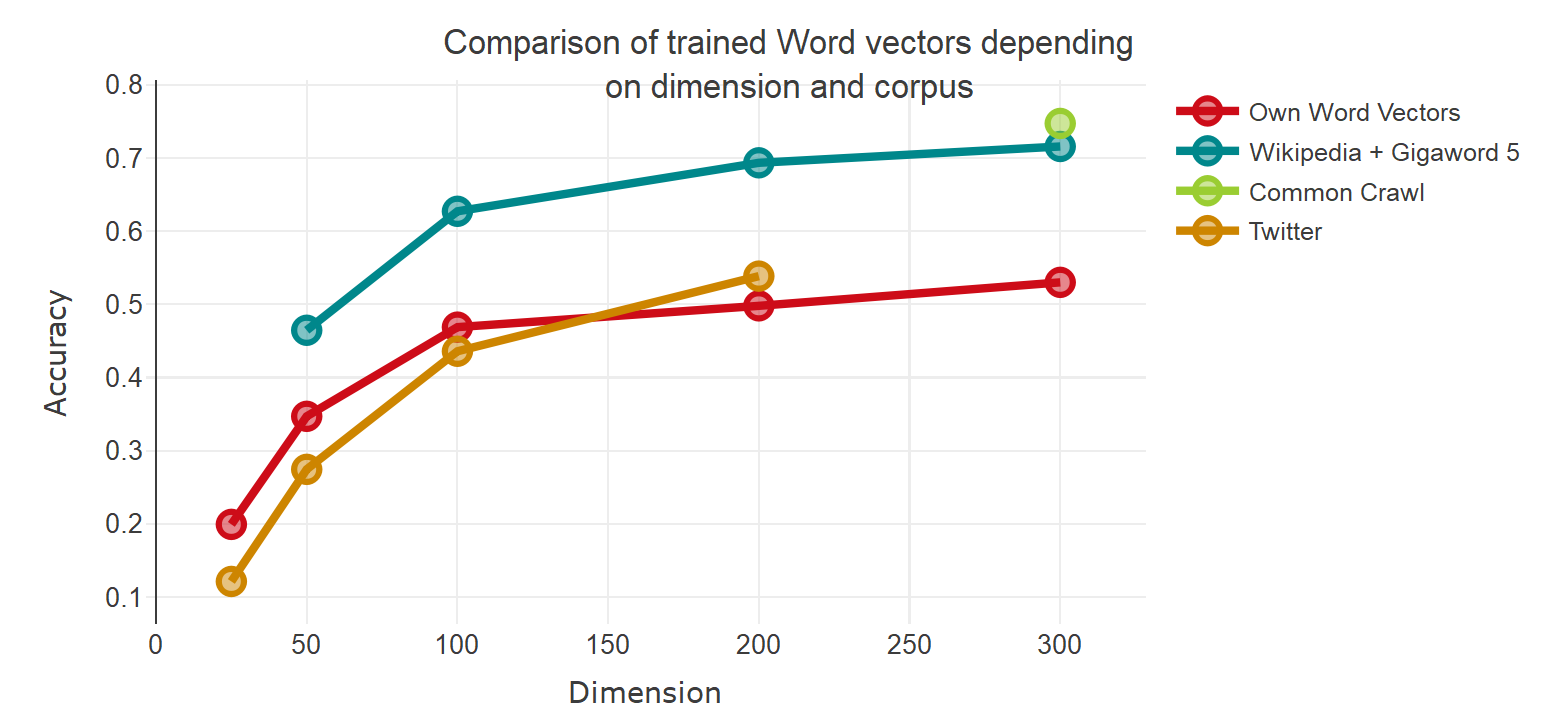
\includegraphics[width=0.9\textwidth]{images/eval_wv.png} 
\caption[Comparison of different word vectors.]{Comparison of the overall accuracy 
         of own word vectors and pre trained word vectors for different dimensions.}
\label{fig:eval-wv}
\end{figure}